\documentclass[12pt,a4paper,oneside]{report}
\usepackage[utf8]{inputenc}
\usepackage[english]{babel}
\usepackage{amsmath}
\usepackage{amsfonts}
\usepackage{amssymb}
\usepackage{graphicx}
\usepackage[left=2cm,right=2cm,top=2cm,bottom=2cm]{geometry}
\author{Daniel Aguiar da Silva Carvalho}
\begin{document}
\sffamily
\begin{center}
\textbf{\large{Thesis Advancement Report 2014-2015 (First Year)}}
\end{center}

\begin{flushleft}
\textbf{Thesis title:} Trusted-SLA Guided on Multi-cloud Environments \\
\textbf{PhD. student:} Daniel Aguiar da Silva Carvalho \\
\textbf{Supervisor:} Chirine Ghedira-Guegan \\ 
\textbf{Co-supervisors:} Nadia Benani and Genoveva Vargas-Solar
\end{flushleft}


\begin{flushleft}
\textbf{Context}\\
\end{flushleft} 

The data integration is a well-known and widely discussed problem in the database area. It consists in merging data from different data sources and granting a unified view of the data~\cite{Lenzerini:2002}. 

Considering this, cloud and multi-cloud computing opens new challenges to data integration. 
The possibility of an unlimited access to resources that arises with the cloud model changes the way to process data.
In this context, some data integration approaches have been proposed.
\cite{Gonzalez:2010b} proposed a cloud-based data management and integration system.
It enables data sharing, integration and collaboration between multiple users. 

%According to some design foundations, such as integration with the web, easy of use, incentives for sharing and facilitate collaboration, the authors described the system  and some examples of applications that can take advantages from it. 

\cite{Gonzalez:2010} described in detail the system architecture, integration process, query processing proposed by~\cite{Gonzalez:2010b}. 
%Additionally, an API and an example of an integrated application with Google Maps is presented. 
\cite{078} combined data integration, service oriented architecture and distributed processing. 
%The Service Oriented Data Integration based on MapReduce System (SODIM) works on a pool of collaborative services and can process a large number of databases represented as web services. 
%
%In the cloud scenario, it is a hard task to one single cloud deliver the resources necessaries to fit customer requirements. 
%To avoid this, cloud providers began to share their computing resources.
%This new (multi)-cloud configuration add more challenges to data integration, considering the large amount and diversity of data, and quality and security aspects of the integration.
%The data privacy is the most tackled aspect in this context.

\cite{YauY08} proposed a privacy-preserving repository in order to integrate data. 
Based on users' integration requirements, the repository supports the retrieval and integration of data across different services. 
\cite{096} introduced an inter-cloud data integration system that considers a trade-off between users' privacy requirements and the cost for protecting and processing data. According to the users' privacy requirements, the query plan in the cloud repository creates the users' query. 

%This query is subdivided into sub-queries that can be executed in  service providers or on a cloud repository.
%Each option has its own  privacy and processing costs.
%Thus, the query plan executor decides the best location to execute the sub-query
%to meet privacy and cost constraints. In general, 
Other quality aspects of data integration services have been highlighted in~\cite{Dustdar:2012}.


In cloud computing, a common way of defining requirements and obligations between the \textit{cloud provider} and \textit{cloud customer} is through service level agreement (SLA) contracts. 
SLAs have been widely adopted in the cloud context. 

\cite{011} presented a approach for security service level agreements on hybrid clouds. The author focus on the lifecycle of a security SLA, considering some security mechanisms (i.e. secure resource pooling, secure elasticity, access control, audit, verification and compliance, and incident management and response).

\cite{009} introduced a generic SLA model that includes management capabilities as a service which are agreed and negotiated in contracts. These management capabilities (elasticity, high availability, scalability and on demand provisioning) are performed by management services called Pcloud services that are defined in order to achieve application requirements. The idea is to help cloud customer to choose the appropriated providers that fits his requirements. 

\cite{005} focused on the designing step of the SLA. 
Based on functional and non-functional requirements of the different cloud delivery models, a conceptual framework for cloud computing is proposed. 
%The objective is to enhance trust and reliability between the parts in the negotiation phase.

Summarizing, the contributions are divided in two groups: (i) approaches focus on the SLA negotiation phase; and (ii) approaches for monitoring and allocation of resources in order to detect and avoid SLA violations. Among them, we identified one single approach regarding data integration in a grid environment guided by SLA~\cite{Nie07}.

We believe that data integration can take advantages by integrating SLA on its solutions. To the best of our knowledge, we have not identified any other proposal adopting the use of SLAs combined with a data integration approach on a (multi)-cloud context.

\begin{flushleft}
\textbf{Problem Statement}\\
\end{flushleft}

We assume that data integration is done on a (multi)-cloud service oriented environment. We also consider that data integration is done under new conditions with respect to the type of data sources, the environment where it is performed and the preferences  of data consumers and the SLA. 
%\begin{figure}[h!]
%\centering
%\includegraphics[scale=0.50]{figs/DataIntegrationContext.pdf} 
%\caption{New data integration context}\label{fig:vision}
%\end{figure}

There are data providers that are services possibly deployed in clouds and available  through their API or in a REST architecture. We assume that  each service exports an agreed SLA that specifies the economic cost per call, the maximum number of calls that can be done per day, the availability of the service, the average response time when a method is called, the reliability, the privacy of the produced data (whether they can be stored or not), the precision of their responses, freshness and provenance of the produced data.  

%\begin{trivlist}\sf\footnotesize
%\item[~$\bullet$ ] {\sf agreedSLA:$\langle$cost/call, maxCalls/day, availability, responseTime, reliability, privacy, precision, freshness, provenance$\rangle$}. 
 %\end{trivlist}


Cloud providers define also their SLA contracts expressing  subscription contracts that specify, the cost per request ({\sf cost/request}), the volume of data that can be exchanged per month ({\sf I/0 volume/month}), the cost of transferring data or applications within the same data centre or between data centres ({\sf datatransferCost/region}), and storage space ({\sf storageSpace}). For example some cloud providers enable the customer to choose the zone to install PaaS services and deploy applications (e.g. zone 1 is Europe). If the customer wishes to deploy services in zone 1 but store data in zone 2 the transfer cost will change.

%\begin{trivlist}\sf\footnotesize
 %\item[~$\bullet$ ]  {\sf cloudSLA:$\langle$cost/request, I/0 volume/month, datatransferCost/region, storageSpace$\rangle$}. 
 %\end{trivlist}


Some of these measures ({\sf cost/call, maxCall/day}) are static and explicitly specified by the service provider. 
In contrast, the other measures should be computed by monitoring the conversations between the service and the applications that contact it.  

In our vision a query expressed in an SQL-like language is associated to a set of QoS preferences expressing the requirements of the user. For example, the economic cost she is ready to pay for executing the query, the provenance of the data, the reputation of data services and the expected time response. The answer of such a query is the result of integrating data from different services according to a series of phases described in the following section.


\begin{flushleft}
\textbf{Hypothesis}\\
\end{flushleft}

We adopted the following hypothesis for defining the methodology of work:

\begin{itemize}
   \item Data integration can take advantages by integrating SLA on its solutions on a (multi)-cloud context;
   \item The key and original aspect of data integration and provision process considering SLA in a (multi)-cloud context can be define a vertical mapping of user QoS preferences and agreed SLAs; 
   \item One possible solution can be define a {\em derived SLA} that guides the evaluation of queries to be executed on the multi-cloud environment; 
   \item Have a framework for it execution can add quality to the integrated solution.

\end{itemize}

\begin{flushleft}
\textbf{Objectives}\\
\end{flushleft}

Based on the aforementioned works and our hypothesis, we are interested in proposing a data integration solution in a multi-cloud environment guided by user preferences and service level agreements (SLA) exported by different clouds. This new approach brings different challenges and open issues. So, the objective of my PhD thesis are:

\begin{itemize}

\item We believe that we can enhance data integration quality by integrating SLA on its solutions. So, To reach this, it is necessary to identify which quality measures associated to data (that the data consumers what to query) and to the multi-cloud context should be present in SLA;

\item Considering the nature of the multi-cloud environment where we dealing with private and public clouds, it is necessary to proposed a mechanism to grant quality and security aspects of the integration to the data consumer;

\item During the integration process, it is also necessary to monitor the SLAs associated to different delivery models in order to avoid violations in the others agreed contracts. So, we will propose a algorithm for that;

\item It is necessary design a new matching-retrieving algorithms in order to perform the integration process, selecting the best service composition according to the user requirements and the SLAs;

\item We will develop a set of algorithms and a framework to reach our target.
\end{itemize}

 
\begin{flushleft}
\textbf{Synthesis and Perspectives of the Research Activities}\\
\end{flushleft}

During the first year of PhD, we have been working on the state of the art. 
The idea is to be aware of all types of publications close related to the thesis proposal. To reach this, we proceeded with a literature analysis using a systematic mapping methodology. 

Briefly, the methodology consists in retrieving papers from scientific databases using the same search string. These papers are filtered according to an inclusion and exclusion criteria that should be defined based on the research interests. The papers will be classified in different categories (called facets) and for each facet in a specific dimension. The facets and dimensions are defined based on the authors knowledge and interests. Taking the final papers collection, the abstracts should be read in order to classify each paper into the dimensions for each facet. 
This methodology allowed us to identify trends and open issues regarding our research topic and proposing an approach that fills some gaps and proposes an original data integration solution according to current trends in the area.

This work performed, we thus have written an article that was \textbf{accepted} to the 26th International Conference on Database and Expert Systems applications (DEXA 2015).
We selected 114 papers based on our inclusion and exclusion criteria. This final data collection builds the state of the art to the thesis and, in the next step, we will perform an in-depth analysis of theses papers in order to (i) analyze what have been made and (ii) propose my approach.  

\bigskip
Based on the publications extracted from the mapping process methodology, we will proceed the analysis of the current state of the art in order to formalize our proposal. The analysis will be the basis to our model proposal. As a natural result, we will write a paper describing our approach and a survey. In parallel, we will carry on the first steps of implementation of the proposed approach.
The figre \ref{fig:calendar} presents the intended calendar. 


\begin{figure}[!h]
\center
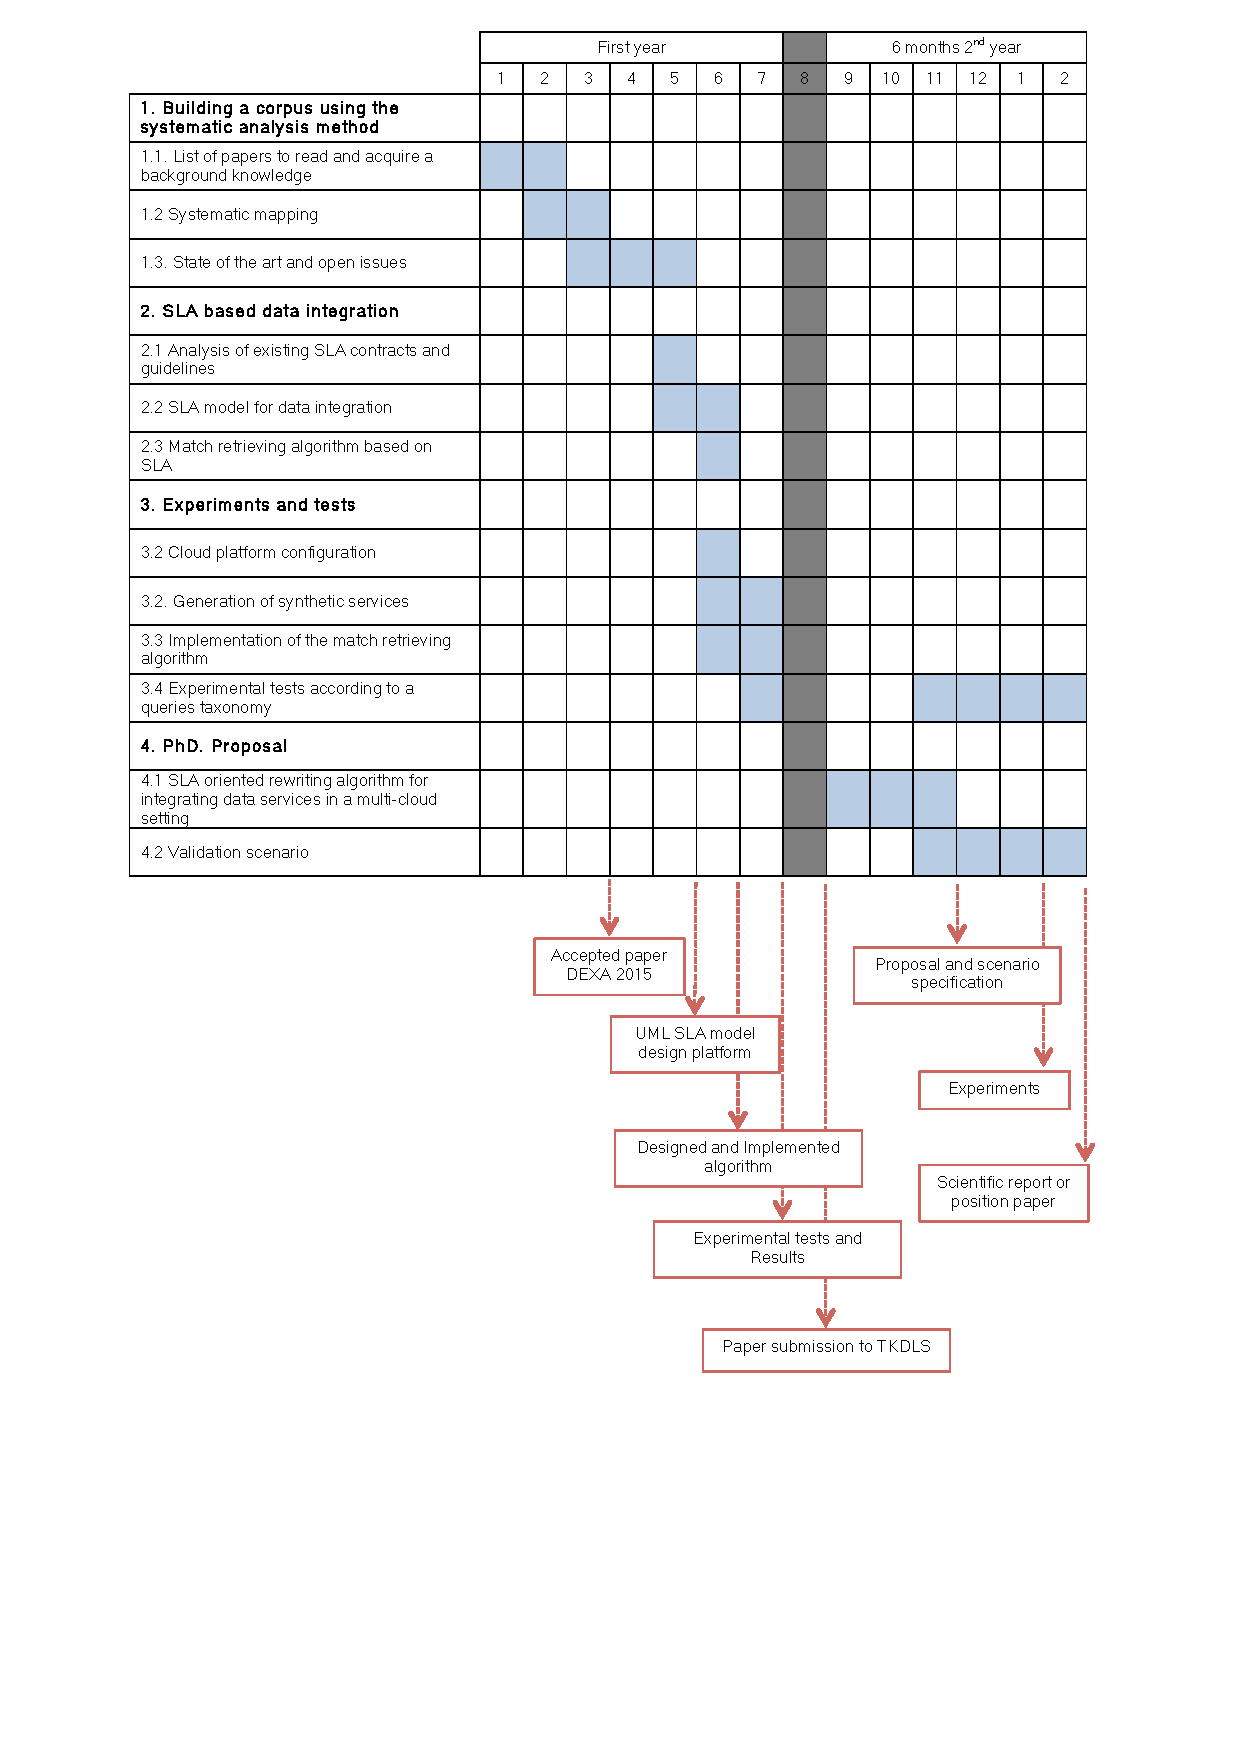
\includegraphics[scale=0.95]{calendario.pdf} 
\label{fig:calendar}\caption{Calendar}
\end{figure}

\bibliographystyle{plain}
\bibliography{bibliography}


\end{document}